\section{Revocation Boundary and Discussion}
\label{sec:discussion}

\subsection{Revocation Freshness: A Negative Result}

The initial concurrency model treated revocation delivery as an atomic resolver-local event. Through bound five, 793,800 event words produced 26,038 executions, 4,534 conflict resolutions, and 1,590 approval timeouts without a delivered-state revocation, permission-union, deterministic-order, or deadlock violation. Exact graph closure for two, three, and four holders converged at depths six, eight, and ten, reaching 1,110 states in total, including 461 states beyond bound five and 10,576 cycle edges, without exposing a new registered violation. These observations established only a local post-delivery boundary.

Separating issuance at the authority service from resolver delivery refuted the preregistered revocation claim, whose registered interpretation is issuance-relative. Each of five fixed scenarios used fair schedules with delay zero, one, or two, and every schedule eventually delivered the revocation. Delay zero produced no stale execution. Delays one and two each produced four, for eight issuance-relative stale executions in total, while all post-delivery and other registered checks remained clean. Fig.~\ref{fig:revocation} shows the resulting window. The counterexamples meet the preregistered false criterion and are not scheduler-nontermination artifacts.

\begin{figure}[t]
\centering
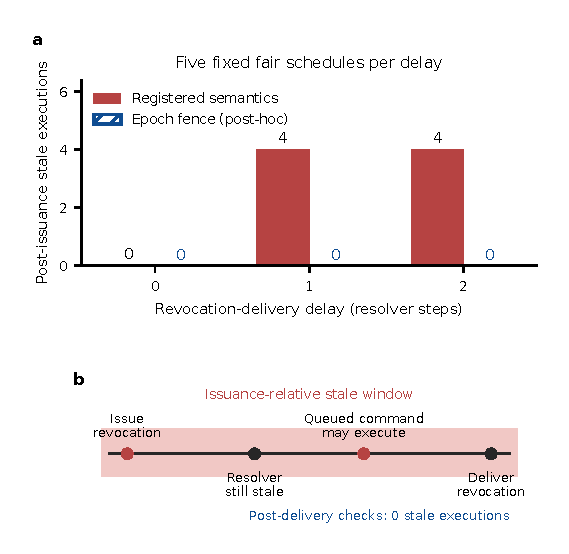
\includegraphics[width=\columnwidth]{figures/generated/fig05_revocation}
\caption{Delayed delivery refutes issuance-relative revocation safety. (a) Each delivery delay contains five fixed fair schedules. The registered semantics produced 0, 4, and 4 post-issuance stale executions at delays 0, 1, and 2, respectively; a post-hoc epoch-fence replay blocked all eight and is shown only as a diagnostic. (b) Revocation issuance opens a stale resolver window in which a queued command may execute before delivery. Every schedule eventually delivered revocation, and no post-delivery stale execution occurred.}
\label{fig:revocation}
\end{figure}

Pinned SINT exhibited the same boundary: before delivery it allowed one stale use and approved one already-queued revoked request, and only a fresh gateway recheck denied execution. An issuer-side epoch fence blocked all eight stale executions in a diagnostic replay. Neither the fence nor the gateway recheck repairs the registered \zonecap{} claim: the fence was introduced after the counterexample, and the SINT check belongs to a separate integration path. They instead identify the missing contract. A local resolver cannot establish issuance-relative safety unless execution is coupled to atomic delivery, a trusted freshness epoch, or a mandatory fresh execution-side check.

\subsection{Implications and Limitations}

The main result is an authorization-refinement interface rather than an intrinsic property of capability syntax. A compiler must establish authorization inclusion, and the runtime layer must establish request-abstracted emission inclusion through sound, parent-realizable outputs. This interface complements capability systems that provide identity, delegation, and cryptographic transport~\cite{dodson2021,dodson2020,sint2026,bamil2026} and runtime enforcers that provide correction, monitor synthesis, and scalable mediation~\cite{pearce2020,lanotte2023,baird2024}. It does not replace controller safety analysis or inherit guarantees that those systems did not claim.

The compiler evidence is intentionally bounded. The compiler and oracle use separate code paths, but both consume a single human-authored interpretation of each source. Provenance probes and mutants reduce shared implementation-error risk, not shared interpretation error. The five behavioral and contextual fields are a source-independent overlay, target assets are deterministic per-zone identifiers, and the ENISA input is a landside-signalling subgraph. The agreement therefore supports the frozen representation and delegation checks; it does not establish completeness for arbitrary IEC~62443 architectures or certification.

The runtime evidence is bounded to actuation events and horizon-five compositions. Real PLC scans advance when no new command is emitted, so fixed-tick integration must define the held output, controller memory, timeout, and plant evolution before re-establishing parent realizability. The current theorem also trusts the physical history, mode, and common plant relation. Compromised sensors, stale context, model mismatch, and asynchronous distributed effects require separate contracts. Finally, the theorem is manually written rather than machine checked, and the baseline projections compare expressible dimensions rather than complete deployed products.

No accepted target-hardware performance evidence is available at the current freeze. The local x86 run validated timer resolution, CPU affinity, forced-slow detection, and six disabled-check controls, but it did not measure the target Jetson Orin NX/OpenPLC path. It cannot support a latency, scan-occupancy, throughput, or memory claim. If the planned target-hardware study later passes its frozen raw-data and equivalence audits, it can be reported as prototype feasibility evidence; until then, the paper makes no performance claim.
